\chapter{Analyzing Language Models: Foundations, Methods, and Tools}
\label{sec:analysis-background}

Understanding how language models learn, represent, and generalize linguistic knowledge requires a diverse set of analytical approaches. This chapter surveys foundational work in three interrelated areas: (1) attention-based and representational interpretability, (2) mechanistic interpretability that aims to reverse-engineer internal computations, and (3) learning dynamics research that tracks how capabilities emerge over time during training. 

Our emphasis is especially on methodologies that provide insight into the internal mechanisms of transformer-based models, with a focus on tools that are most relevant to understanding small models and their developmental trajectories. Throughout the chapter, we highlight key techniques for probing attention heads, decomposing learned circuits, tracking convergence and capacity usage, and analyzing models across training checkpoints and scales.

We also introduce the growing ecosystem of open-source model suites and analysis frameworks that enable this work—resources that make it possible to observe, quantify, and intervene in learning dynamics directly. These tools will form the empirical and methodological foundation for the contributions in the next chapters, where we analyze how small models diverge from larger ones and propose interventions to improve their learning behavior.
\section{Analysis of Attention}

The transformer architecture brought the attention mechanism to the forefront of representation learning. Early efforts to interpret these models focused on analyzing attention patterns to uncover what linguistic information models capture and how it is distributed across their components.

\subsection{Multi-Head Attention Analysis}

Early efforts to understand transformer models focused heavily on analyzing attention patterns—both to probe internal representations and to assess model efficiency.

A foundational study by \citet{voita2019analyzing} showed that attention heads in transformer models often specialize in distinct linguistic roles, such as syntactic dependencies, coreference, and discourse relations. This head-level specialization pointed to an emergent modularity, where different heads implicitly divide up the task of language processing.

Crucially, they also demonstrated that many heads could be pruned with minimal impact on downstream performance, suggesting that only a subset are essential. This insight laid the groundwork for head pruning as a principled form of model compression.

\citet{michel2019sixteen} expanded on these findings by empirically measuring redundancy among attention heads. They showed that despite being designed for parallel attention, many heads capture overlapping information, reinforcing the sparsity hypothesis and motivating leaner transformer designs.

Building on these analytical approaches, \citet{clark2019does} developed visualization methods for interpreting attention in BERT. Their study found that BERT's attention heads capture both syntactic and semantic relationships—for instance, tracking subject-verb agreement or coreference chains. This work helped establish attention weights as interpretable proxies for internal reasoning, turning attention visualization into a widely used diagnostic tool in transformer research.

\subsection{Sparse Probing}

While attention-based methods offer a window into model behavior, other approaches have investigated how linguistic structure is embedded in hidden representations. \citet{hewitt2019structural} introduced a structural probe to test whether contextual embeddings encode syntactic information such as dependency trees. Their results showed that BERT's middle layers encode rich syntactic structure in a geometrically meaningful way, revealing that grammar is implicitly embedded in the model's representational space.

More recently, \citet{gurnee2023finding} proposed sparse probing—a technique that constrains linear probes to use only a small number of neurons, enforced via $L_0$ regularization. Their results suggest that linguistic features, while broadly distributed, can be reliably recovered from sparse subsets of neurons. This highlights the potential for localized interpretability, particularly relevant for small models where transparency is more attainable.

\section{Mechanistic Interpretability}

While sparse probing offers a high-level view of which neurons encode linguistic features, mechanistic interpretability aims to reverse-engineer how those features are computed—tracing internal mechanisms such as circuits, neurons, and layer interactions that give rise to model behavior.

\subsection{Foundational Ideas and Circuits}

\begin{figure}[ht!]
    \centering
    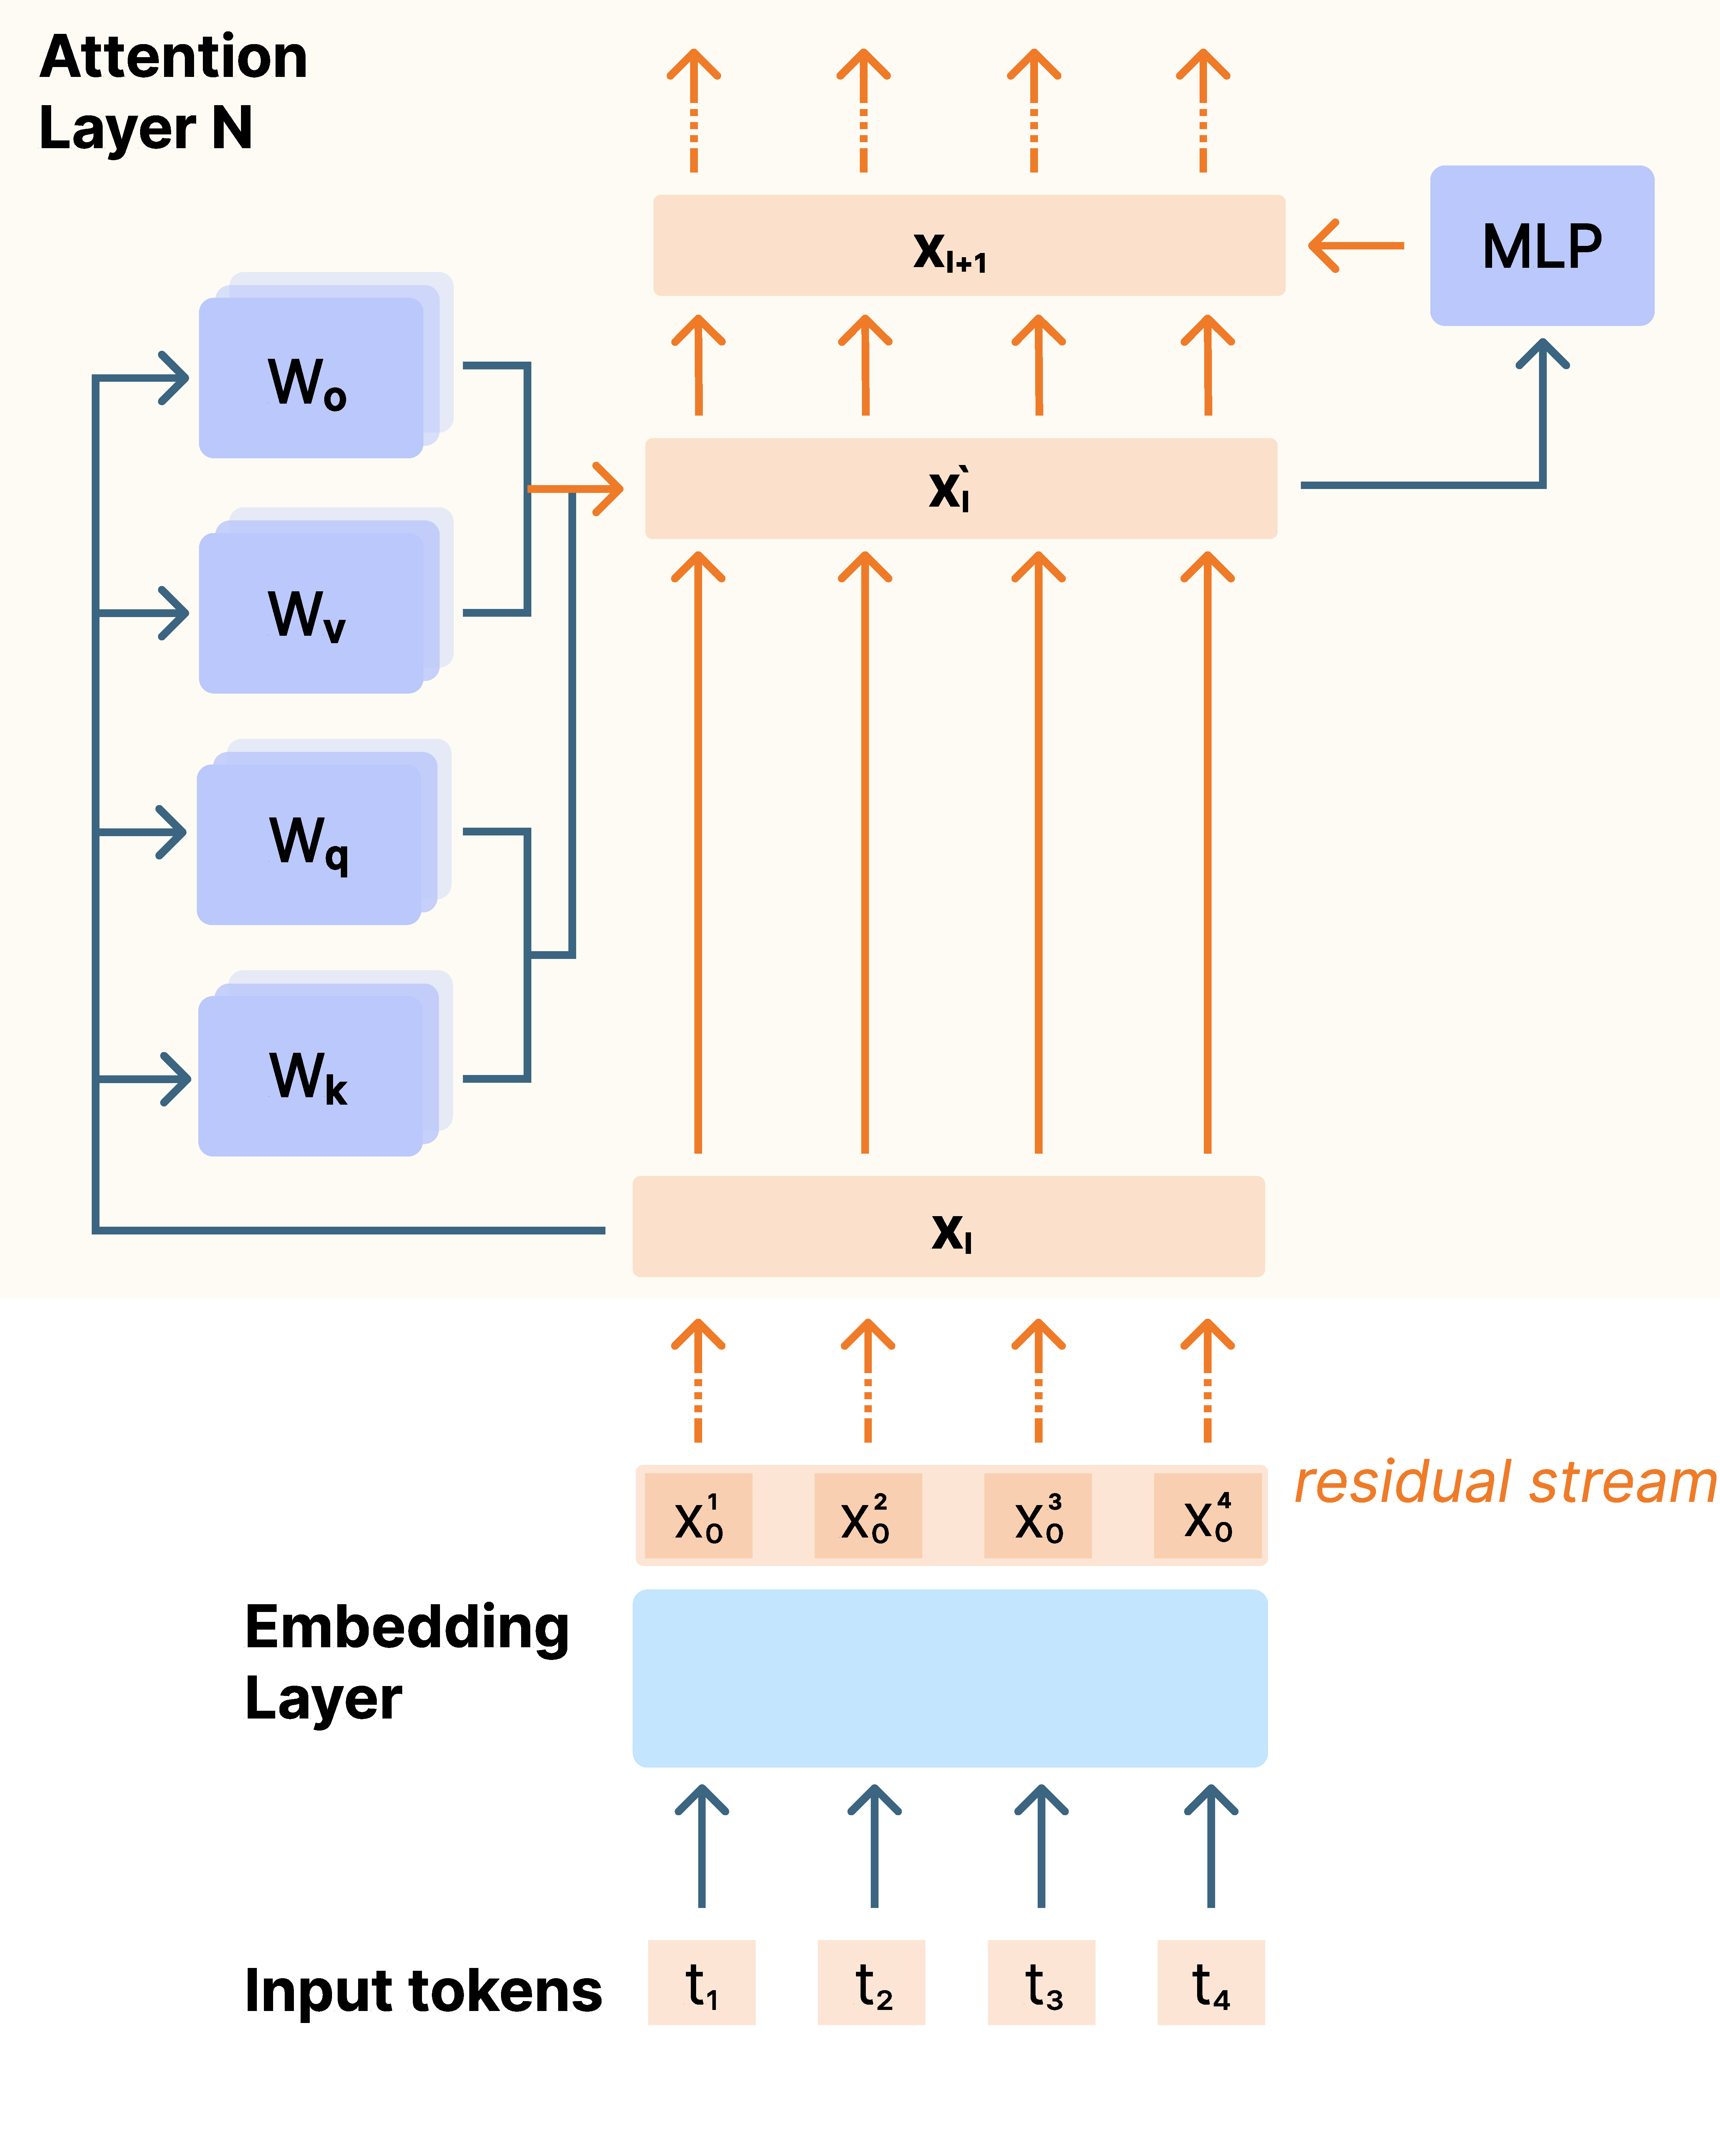
\includegraphics[width=0.6\textwidth]{chapters/analysis_background/figures/residual_stream_visualization.pdf}
    \caption{Visualization of the residual stream in a transformer model, showing how information flows through the network via skip connections and is progressively refined through attention and feed-forward layers.}
    \label{fig:residual-stream}
\end{figure}


The theoretical foundations of this field were laid by \citet{olah2014manifolds}, who framed neural networks as systems that deform data manifolds while preserving topological structure. This perspective provides a conceptual basis for interpreting how deep models process and transform information layer by layer.

Building on this, \citet{elhage2021mathematical} introduced a formal framework for decomposing transformers into interpretable circuits. Using tools like “virtual weights,” they showed how specific attention heads can implement distinct algorithms—such as copying or positional induction—forming structured computational graphs within the model. These operations are executed within the shared residual stream, a central component of transformer architecture that carries forward and combines layer outputs across the model.

The residual stream is a mathematical formalization through which to study how transformer models process inputs \citep{elhage2021mathematical}. Under this framework, each of the $L$ layers of a transformer model processes a series of input tokens $\sequence = \langle \token_1, \smalldots, \token_\seqlen\rangle$ consecutively and communicates the result of its computation for each token to subsequent layers via a residual stream of dimension $\residualdim$. 

The reading, processing, and writing of the residual stream occur independently in each $\attention$ head via combinations of the query, key, value, and output matrices, $W_Q$, $W_K$, $W_V$, $W_O$. The \textbf{query-key circuit}, $W_Q^{\top}W_K$, of the $\attention$ mechanism controls how the residual stream should be recomposed, and the \textbf{output circuit}, $W_OW_V$, writes to the residual stream an update that is mediated by the query-key circuit. The write operation of each $\attention$ head is of low rank relative to $\residualdim$. After each $\attention$ head has written to the residual stream, a bottleneck $\mlp$ projection performs a full-rank transformation on the residual stream. Due to their pivotal role in updating the state of the residual stream, our work analyzes the learning dynamics of the two operations that write to the residual stream: the output circuit of each head of the $\attention$ layer---that we refer to as $\attention$---and the $\mlp$ projection layer---that we denote $\mlp$ for conciseness.

As illustrated in \cref{fig:residual-stream}, the residual stream serves as the backbone of computation, enabling attention and feed-forward layers to progressively refine and update internal representations at each layer.

A key example of this modular behavior is the “induction head” described by \citet{olsson2022inductionheads}, which performs in-context learning by detecting repeating token patterns. Their work demonstrated that induction heads are universal across transformer models and emerge consistently during training, highlighting how meaningful algorithmic structure can arise within the residual stream.

\subsection{Representation, Superposition, and Memory}

Neural networks often represent multiple features in overlapping activation dimensions—a phenomenon known as superposition. \citet{elhage2022toy} formalized this idea and showed how it creates both efficient storage and representational interference. They proposed sparse coding as a way to reduce overlap and improve interpretability.

Complementary work by \citet{geva2021memory} reframed feed-forward layers as key-value memory stores, where neurons act as retrievable content-addressable memories. This perspective highlights how information retrieval occurs outside the attention mechanism, reshaping our understanding of transformer architecture.

\citet{dai2022knowledge} further explored how factual information is stored in “knowledge neurons”—units that encode specific facts in a distributed but partially localizable way. These findings reinforce the idea that interpretability is possible even in large, dense models, particularly through targeted neuron analysis.

\subsection{Toward Full Decomposition}

Recent efforts have focused on decomposing model activations into monosemantic features—components that represent a single, interpretable concept. \citet{bircken2023monosemanticity} applied sparse autoencoders to learn such features from model activations, revealing interpretable directions in activation space. This method shows promise for mitigating superposition and improving transparency.

\citet{anthropic2023components} outlined a broader research vision for full model interpretability, where each parameter's role is understood. Their approach leverages dictionary learning and modular decomposition to identify circuits, features, and neurons aligned with human-understandable behaviors.

\subsection{Tools for Intermediate Layers and Model Analysis}

To support these interpretability efforts, a range of tools and frameworks have emerged.

\citet{belrose2023eliciting} developed the Tuned Lens, an extension of the logit lens, which improves interpretability of intermediate layers by learning linear probes that better approximate the model's output predictions at earlier stages. This allows for clearer analysis of how information evolves through the network.

\citet{nanda2022transformerlens} introduced TransformerLens, a library for inspecting transformer internals—including attention heads, MLP layers, and residual streams. It is widely used for circuit-level analysis, enabling researchers to trace forward and backward signals through static, trained models.

Several tools also support causal and structural interventions. \citet{meng2022locating} proposed ROME, a technique for directly editing factual knowledge in a trained transformer by locating and modifying causal neurons. Similarly, \citet{conmy2023towards} developed ACDC, which uses sparse matrix factorization to automatically extract circuits from models, enabling inference-time interpretability without retraining.

For broader attribution analysis, \citet{kokhlikyan2020captum} developed Captum, a general-purpose library for feature attribution in PyTorch. While not transformer-specific, it includes a suite of interpretability tools—such as Integrated Gradients and DeepLIFT—that are useful for probing feature importance across different model architectures.

% \section{Developmental Interpretability}
% While mechanistic interpretability reveals the internal structure of trained models, developmental interpretability shifts focus to how those structures emerge during training. By analyzing checkpoints over time, this approach captures the trajectory of learning—offering insight into when and how linguistic capabilities arise.

% \citet{hoogland2023towards} introduced this paradigm by identifying phase transitions in learning, supported by the Local Learning Coefficient as a measure of representational complexity. Building on this, \citet{hoogland2025losslandscape} connected stagewise learning to loss landscape geometry, revealing that shifts in capability often align with flat or degenerate regions in the optimization surface.

% To support empirical analysis, \citet{devinterpcode} developed DevInterp, a toolkit for tracking model development over time. Together, these contributions establish developmental interpretability as a powerful complement to static and circuit-based approaches—highlighting not just what models learn, but when and how they acquire it.

% This developmental perspective naturally leads into a broader field of inquiry: learning dynamics—the study of how language models acquire, retain, and organize knowledge over time.

\section{Developmental Interpretability}
While mechanistic interpretability reveals the internal structure of trained models, developmental interpretability shifts focus to how those structures emerge during training. By analyzing checkpoints over time, this approach captures the trajectory of learning—offering insight into when and how linguistic capabilities arise.

\citet{hoogland2023towards} introduced this paradigm by identifying phase transitions in learning, supported by the Local Learning Coefficient as a measure of representational complexity. Building on this, \citet{hoogland2025losslandscape} connected stagewise learning to loss landscape geometry, revealing that shifts in capability often align with flat or degenerate regions in the optimization surface.

To support empirical analysis, \citet{devinterpcode} developed DevInterp, a toolkit for tracking model development over time. Together, these contributions establish developmental interpretability as a powerful complement to static and circuit-based approaches—highlighting not just what models learn, but when and how they acquire it.

This developmental perspective naturally leads into a broader field of inquiry: learning dynamics—the study of how language models acquire, retain, and organize knowledge over time. But developmental interpretability is just one part of a broader movement toward training-time analysis. To fully understand how language models acquire and organize their capabilities, we need a more expansive view—one that considers not just phase transitions, but also how examples are memorized or forgotten, how representations converge, how capacity is allocated, and how internal structures evolve in rank and geometry.

\section{Learning Dynamics Research}

Understanding how language models learn—beyond just what they ultimately represent—is central to both interpretability and model development. Learning dynamics research investigates the evolving internal behavior of models throughout training, revealing how linguistic capabilities emerge, stabilize, or fail to develop.

This work spans a diverse set of analytical perspectives, each offering insights into different facets of training-time behavior.

\subsection{Memorization and Data Influence Analysis}

A central goal in learning dynamics is to understand how specific examples affect learning over time—whether they are memorized, generalized, or forgotten.

Influence functions, introduced by \citet{koh2017understanding}, trace the effect of individual training examples on model predictions by approximating parameter updates through gradients and inverse Hessians. \citet{grosse2023influence} extended this method to large language models, enabling counterfactual analysis: how would the model behave if a given sequence were added to the training set?

Complementary to this, prediction trajectory methods analyze how model outputs evolve across training steps. \citet{toneva2019empirical} introduced the concept of forgetting events—when a model switches from correct to incorrect on a training example—offering a lens on stability and difficulty. \citet{swayamdipta2020dataset} expanded this idea with dataset cartography, classifying examples by prediction confidence and variability to map learning trajectories across NLP datasets.
\citet{feldman2020does} examined the tradeoff between memorization and generalization, especially in smaller models where memorization may be necessary for strong performance. \citet{biderman2023emergent} investigated verbatim memorization in the Pythia model suite, finding that early checkpoints can effectively forecast what large models will eventually memorize—though smaller models cannot.

Together, these approaches reveal that memorization is shaped by training dynamics, model scale, and the specific properties of the data.

\subsection{Convergence and Representation Similarity}

While memorization-focused analyses emphasize how individual examples influence a model's behavior, convergence analysis shifts attention to the evolution and stabilization of internal representations during training. This research area seeks to understand when and how model layers begin to encode stable linguistic abstractions, how representational structures develop over time, and the extent to which different models (trained on the same or different data) develop similar internal solutions.

\subsubsection{Measures of Representational Similarity}

A foundational family of methods in this space builds on \textit{Canonical Correlation Analysis (CCA)}, which compares the similarity between two multivariate representations. In neural networks, this allows researchers to quantify the alignment between layer activations at different checkpoints, across different models, or within different layers of the same model. \citet{raghu2017svcca} introduced \textit{Singular Vector CCA (SVCCA)}, which first reduces the dimensionality of representations via singular value decomposition before applying CCA to the resulting principal components. This makes the method more robust to noise and scale differences in deep representations. However, SVCCA has limitations in terms of sensitivity and interpretability.

To address these limitations, \citet{morcos2018pwcca} proposed \textit{Projection-Weighted CCA (PWCCA)}, which weights the contribution of each component according to how much it aligns with the original data. This technique down-weights noisy or low-signal components, yielding a more faithful measure of similarity. Despite these refinements, CCA-based methods still struggle in settings where the representation dimensionality exceeds the number of datapoints---a common scenario in large-scale models with deep layers and high-dimensional embeddings.

To overcome this, \citet{kornblith2019cka} introduced \textit{Centered Kernel Alignment (CKA)}, a method based on kernel similarity that offers greater robustness across dimensional regimes. In its linear form, CKA computes the similarity between two activation matrices \( X, Y \in \mathbb{R}^{n \times d} \) as:

\[
\mathrm{CKA}(X, Y) = \frac{\| Y^\top X \|_F^2}{\| X^\top X \|_F \cdot \| Y^\top Y \|_F}
\]

where \( \|\cdot\|_F \) denotes the Frobenius norm. This measure is invariant to orthogonal transformations and isotropic scaling of the representations, making it well-suited for comparing different models or different training stages. CKA has since become a standard tool for tracking representational convergence in both vision and language models.

While CKA and CCA focus on representational similarity in a static sense, another approach---\textit{model stitching}---investigates whether different models are \textit{functionally} equivalent at certain layers. Originally proposed by \citet{lenc2015understanding} for convolutional networks, this method was later formalized by \citet{bansal2021stitch} as a technique for connecting the lower layers of one model to the upper layers of another, using a small trainable adapter in between. If the stitched model performs well, it suggests that the internal representations of the two models are sufficiently aligned to be interoperable. Stitching provides a more dynamic view of convergence, capturing not just alignment in activation space but also compatibility in downstream processing.

\subsubsection{Applications to Language Models}

These methods have been extensively applied to \textit{language models} to understand the progression and stability of learned representations. For instance, \citet{saphra2019understanding} used SVCCA to track the alignment of ELMo's hidden states with syntactic annotations, finding that parts-of-speech (POS) information is learned early in training and primarily encoded in lower layers. Similarly, \citet{singh2019bert} applied CCA to multilingual BERT and discovered that representations in the deeper layers diverge across languages, forming hierarchical clusters that reflect known linguistic relationships---suggesting that BERT learns distinct structural priors for different languages.

More recent work by \citet{nguyen2020wide} and \citet{phang2021finetuned} used CKA to identify \textit{block structure} within deep transformers, where layers cluster into groups that share similar representations. These structures are especially pronounced in larger models and later in training, where adjacent layers often encode similar abstractions. \citet{wu2020similarity} found that models from the same architecture family tend to exhibit stronger representational similarity, even if individual neurons vary---suggesting shared inductive biases across architectures. Finally, \citet{brown2023understanding} analyzed intra- and inter-model similarity within the Pythia model suite, using CKA to identify both convergence points and divergence in representation trajectories over time. Their findings support the idea that convergence is not uniform across training but rather unfolds in stages that reflect changes in capacity utilization, generalization, and abstraction.

In summary, convergence analysis provides a global view of how language models evolve during training---not at the level of individual examples, but at the level of their internal geometry. Techniques such as CKA, PWCCA, and model stitching offer complementary insights into how and when models develop aligned representations, how stable those representations are, and to what extent learned abstractions are transferable. These tools are especially valuable in the study of small models, where transparency and structure are more accessible and where representational convergence can serve as a guide for diagnosing inefficiencies, bottlenecks, or missed opportunities in training.

\subsection{Sparsity and Norms Analysis}

While convergence analysis provides a high-level view of how internal representations stabilize over time, another important dimension of learning dynamics concerns how models manage and allocate their \textit{capacity}—both in terms of which parameters are used and how their magnitudes evolve. Analyses of \textit{sparsity} and \textit{norms} offer fine-grained insight into how models compress information, avoid redundancy, and maintain stable training.

This line of work investigates not only how sparsity emerges during training, but also how different types of norms—such as activation norms, weight norms, and gradient scales—fluctuate and influence model behavior. Together, these metrics help reveal how language models balance expressivity with efficiency and stability.

\subsubsection{Sparsity Metrics and Analysis}

A foundational contribution to the measurement of sparsity came from \citet{hoyer2004sparsity}, who proposed a continuous sparsity score that combines the \( \ell_1 \) and \( \ell_2 \) norms of a vector. This \textit{Hoyer's sparsity} metric ranges from 0 (fully dense) to 1 (maximally sparse), making it particularly effective for tracking the emergence of sparse representations in activation maps or weight matrices during training. Its simplicity and interpretability have made it widely adopted in analyzing deep networks, including transformers.

\citet{hurley2009gini} evaluated various sparsity measures from a theoretical perspective, outlining six desirable properties such as scale and permutation invariance. They showed that both the Gini coefficient and Hoyer’s metric satisfy these criteria, validating their robustness for analyzing sparsity in neural models.

\subsubsection{Functional Sparsity in Language Models}

Beyond abstract metrics, several studies have explored \textit{functional sparsity}: how neural models naturally deactivate or underutilize certain components during training. \citet{frankle2019lottery} introduced the \textit{lottery ticket hypothesis}, showing that sparse subnetworks within overparameterized models can achieve full performance if trained in isolation. This finding sparked a wave of interest in understanding which parameters are actively contributing to learning and which are not.

Building on this, \citet{michel2019sixteen} found that many attention heads in transformers can be pruned without degrading performance—suggesting redundancy in head usage and an opportunity for model compression. \citet{voita2019analyzing} confirmed this by introducing \textit{head importance scoring}, showing that some attention heads specialize in interpretable functions while others effectively deactivate, illustrating emergent sparsity during training.

\citet{evci2020rigging} analyzed the training trajectories of sparse networks and found that early training phases are especially unstable when sparsity is enforced too aggressively. This underscores the importance of understanding when sparsity is beneficial and how it interacts with training dynamics.

More recently, \citet{jiang2023pruning} proposed sparsity-aware pruning strategies tailored to pretrained transformers, focusing on neurons that become saturated, unused, or ``dead'' over the course of training. Their work provides practical tools for diagnosing inefficiencies in model capacity usage.

\subsubsection{Norm Evolution and Training Stability}

Complementing sparsity analysis, research into \textit{norm dynamics} offers insight into the scaling and stability of model parameters and activations. \citet{mishkin2016goodinit} studied how weight and activation norms evolve during training and highlighted the role of proper initialization and normalization (e.g., LayerNorm) in maintaining stable learning. Their findings are particularly relevant in transformer architectures where residual pathways can lead to norm drift.

\citet{liu2020understanding} examined \textit{gradient and activation norm instability} in transformers, identifying early-phase training as especially vulnerable to vanishing or exploding norms—an issue especially pronounced in smaller models. These instabilities can explain training failures and motivate adjustments to learning rates, normalization, or initialization strategies.

From a theoretical angle, \citet{arora2018theoretical} connected parameter norm growth to generalization bounds, suggesting that norm-based proxies can signal overfitting or underfitting. Meanwhile, \citet{zhang2021calibration} studied \textit{logit norms} as a proxy for model confidence, showing that poorly calibrated models tend to have misaligned norm dynamics at the output layer. Their findings highlight how monitoring output norm evolution can inform assessments of prediction reliability during training.


\subsection{Rank and Geometry Analysis}

Beyond parameter count or loss metrics, understanding how many dimensions a model \textit{actually uses} to represent information reveals important dynamics of learning and capacity utilization. Rank and geometry analysis captures how representational complexity evolves during training, identifies learning phase transitions, and highlights inefficiencies in model design—particularly in small or overparameterized models.

Training often unfolds in distinct stages, each marked by shifts in representational rank. \citet{boix-adsera2023rank} showed that transformer weights increase in rank incrementally from initialization, mirroring stepwise acquisition of complexity. \citet{belrose2024neural} further observed that models progressively encode more sophisticated statistical patterns—starting from unigrams and advancing toward syntax—suggesting stagewise curriculum-like learning.

Structural limits also constrain learning. \citet{godey2024small} found that small language models hit a representational bottleneck at the output layer: the softmax saturates in rank even while loss continues to fall. This suggests underperformance may stem from expressivity ceilings, not optimization failure.

To characterize these dynamics, researchers have proposed several ways to estimate how many dimensions a model \textit{functionally} uses. \citet{garg2025utilizedrank} introduced \textit{utilized rank}, which estimates the number of active dimensions in a layer's weight matrix by projecting it onto input/output subspaces derived from real data. Their analysis showed that many large models use only a small fraction of their nominal capacity—e.g., ViT-L/16 utilizes just $\sim$20\% of its available rank.

Another approach is \textit{effective rank} (ER), a continuous measure of dimensionality based on the entropy of a matrix's singular values \citep{roy2007effectiverank}. Given singular values $\sigma_1, \dots, \sigma_r$, normalized as $p_i = \frac{\sigma_i}{\sum_j \sigma_j}$, of a matrix $\mathbb{A}$, the effective rank is defined as:

\[
\mathrm{ER}(A) = \exp\left(-\sum_{i=1}^r p_i \log p_i\right)
\]

This metric ranges from 1 (collapsed representation) to $r$ (full rank), offering a smooth, interpretable way to track representational complexity. We adopt this measure in later chapters to analyze the learning dynamics of small language models.

Multiple studies have observed discrete jumps in effective rank, closely aligned with drops in training loss—a phenomenon termed the \textit{rank staircase} by \citet{yang2024rankstaircase}. These transitions mark key inflection points in the learning process, supporting the idea that training progresses in qualitatively distinct stages.

More broadly, rank-based analyses suggest that low-rank structure is an emergent property of training itself. \citet{pellegrino2023lowrank} found that both biological and artificial networks tend to evolve along low-dimensional subspaces. \citet{feng2022rank} and \citet{minyoung2022lowrank} provide theoretical support, showing that neural networks exhibit a bias toward rank-deficient representations and structurally simple solutions.

In sum, rank and geometry analysis deepens our understanding of how language models acquire, compress, and allocate representational capacity. These tools shed light on inefficiencies in training and architecture and serve as valuable diagnostics for learning progression. Later chapters build on this foundation, using effective rank to study capacity bottlenecks and phase transitions in small model training.

\section{Frameworks and Tools for Learning Dynamics Research}

Understanding how language models learn requires visibility into the training process itself. This is especially critical when comparing how models of different sizes acquire capabilities, converge to solutions, or fail to do so. Smaller models often underperform not because of optimization failure, but due to structural limitations and divergence in learning trajectories. To study these differences, researchers increasingly rely on model suites that expose internal states over time and across scales.

This section surveys a set of frameworks that make such investigations possible. These resources are essential for answering \textbf{Research Question 2:} \textit{How can we more quantitatively understand how small models learn and what makes them different from large models?} By enabling cross-scale comparisons, these tools help reveal when and why smaller models diverge, and support targeted hypotheses for making their learning dynamics smoother and more effective.

\subsection{Comprehensive Model Suites with Scale Transparency}

One of the most widely used resources for studying learning dynamics is \textit{Pythia} \citep{biderman2023pythia}, a suite of 16 decoder-only language models ranging from 70M to 12B parameters. Each model includes 154 training checkpoints, enabling fine-grained analysis across both time and scale. Pythia has become a standard resource for studying memorization, convergence patterns, and representational development in autoregressive transformers.

OLMo \citep{groeneveld2024olmo} builds on this trajectory with a focus on full-stack transparency and controlled experimentation. It includes several 7B-parameter models and a 1B model, all trained on 2T tokens with full access to training logs, intermediate checkpoints, and evaluation tools such as Catwalk and Paloma. By standardizing optimization settings and infrastructure, OLMo supports research into scaling laws, optimization dynamics, and reproducible model development.

Complementing this, BLOOM \citep{le2023bloom} offers a multilingual and globally inclusive model suite. It spans models from 560M to 176B parameters, with public checkpoints released at multiple stages (e.g., 100B, 500B, 1.5T tokens). BLOOM is particularly well-suited for studying cross-lingual representation learning and transfer, making it a valuable resource for multilingual language modeling research.

In parallel, LLM360 \citep{liu2023llm360} takes a radical transparency approach by releasing dense sequences of checkpoints—360 for Amber and 143 for CrystalCoder—alongside optimizer states, loss curves, and detailed logs. This level of granularity supports fine-grained studies of model robustness, generalization, and representational change across training.

\subsection{Frameworks for Small Model Interpretability}

Several recent frameworks have focused on smaller, more interpretable models. \textit{MobiLlama} \citep{thawakar2024mobillama} provides a lightweight GPT-style model trained with full transparency and reproducibility, emphasizing efficiency and training traceability for mobile use cases. \textit{TinyLlama} \citep{liu2023llm360} offers a 1.1B-parameter model trained on 3T tokens, with checkpoints released at regular intervals (105B to 3T tokens). Finally, \textit{SmolLM2} was specifically designed for mechanistic interpretability with native Hugging Face integration, releasing checkpoints every 125K steps from a 1.7B-parameter model. 

\subsection{Implications for Learning Dynamics Research}

Collectively, these frameworks provide the empirical foundation for learning dynamics research by exposing how models evolve over time and across scales. With access to intermediate checkpoints, logs, and multiple model sizes, they enable systematic comparisons of when and how capabilities emerge—and why smaller models often diverge from their larger counterparts.

In the next chapter, we use the Pythia suite to analyze differences in convergence between small and large models, motivating hypotheses about how to encourage smoother learning. Building on these insights, the final chapter introduces \textit{Pico}, a new framework designed to support efficient, interpretable retraining of small models and accelerate experimental iteration on learning dynamics interventions.
